

\begin{figure*}[ht]
  \vspace{-10pt}
   \begin{minipage}[b]{\textwidth}
  % \begin{center}

    \subfigure[aligned MHC pangenome]{
      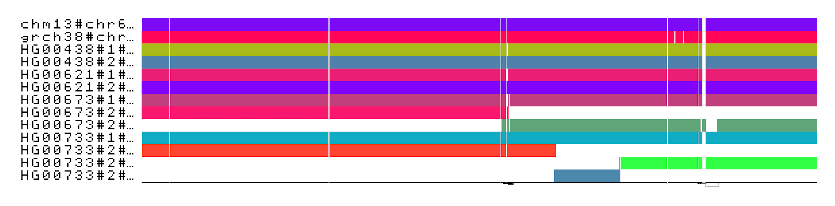
\includegraphics[width=.48\textwidth]{fig/mhc-align.eps}
      \label{subfig1}
    }
    \vspace{-11pt}
    % \newline
    \subfigure[consensus MHC pangenome]{
      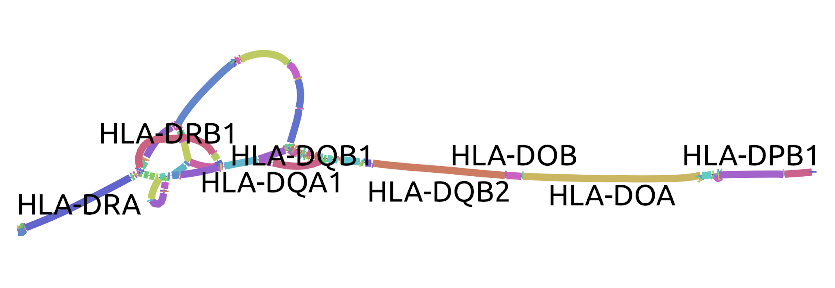
\includegraphics[width=.48\textwidth]{fig/mhc-pangenome.eps}
      \label{subfig2}
    }
    \caption{Examples of output generated by \odgi\ visualizing the
      Major Histocompatibility Complex (MHC) \textit{locus}. (a)
      \cmd{odgi viz} projection of full MHC of eight haploid phased
      human genome assemblies, plus the chm13 cell line and GRCh38
      reference genomes as supplied by the human reference pangenome
      consortium\citep{RPC}. The coloured bars represent the
      linearized paths --- representing individuals --- as a zoomed
      out multi-sequence alignment. The black lines at the bottom
      represent the graph topology. (b) consensus representation of
      the graph of the same MHC assemblies showing variations larger
      than $100$ base pairs. The gene label coordinates were super
      imposed by \cmd{odgi position} from GRCh38. Figure genrated by
      the Bandage tool\citep{26099265} }

  % \end{center}
  \end{minipage}
\end{figure*}
